\chapter{Classes and Objects}
These days, everything is
\href{http://en.wikipedia.org/wiki/Object-oriented_programming}{\emph{object-oriented}}.  
After having spotted
\href{http://www.danielsen.com/jokes/objecttoaster.txt}{object oriented toasters}  
on the loose, we have decided that \textsc{SetlX} should not be an exception.  Therefore,
\textsc{SetlX} supports some basic means for object oriented programming.  Most importantly,
\textsc{SetlX} supports classes.  In \textsc{SetlX} a  
\href{http://en.wikipedia.org/wiki/Class_(computer_programming)}{\emph{class}}
is an agglomeration of variables and functions.  These variables are referred to as 
\emph{member variables}, while the functions are called \emph{methods}.  
In this chapter we demonstrate how classes can be defined and used in \textsc{SetlX}.  
However, this chapter is \underline{not} intended to be an introduction into object-oriented
programming.  Therefore,  we assume that the reader 
has had some previous exposition to object oriented programming in a language like \textsl{Java} or
\texttt{C++}.   In the first section of this chapter, we give some simple examples of class definitions.
The programs presented in that section are not intended to compute anything usefull.  Their
purpose is just to demonstrate the basic features of object-oriented programming that are available
in \textsc{SetlX}.  The second  and third subsection will then discuss more interesting examples:
The second subsection shows how to implement weighted directed graphs via classes and the final
subsection discusses the implementation of complex numbers.  The final subsection will also discuss
some of the more advanced features of object-oriented programming that are available in
\textsc{SetlX}.  In particular, we will discuss operator overloading.

\section{Basic Examples}
In this section, we introduce the basic means by which object-oriented programming is supported in
\textsc{SetlX}.  In the first subsection, we introduce classes.  The second subsection shows how to
simulate inheritance.

\subsection{Introducing Classes}
Our first example deals with the representation of points in a plane.  One way to specify a point
$p$ is to specify both its $x$ and its $y$-coordinate.  This leads to the class definition shown in
Figure \ref{fig:point.stlx} on page \pageref{fig:point.stlx}.  We discuss the details of this
definition next.

\begin{figure}[!ht]
\centering
\begin{Verbatim}[ frame         = lines, 
                  framesep      = 0.3cm, 
                  firstnumber   = 1,
                  labelposition = bottomline,
                  numbers       = left,
                  numbersep     = -0.2cm,
                  xleftmargin   = 0.8cm,
                  xrightmargin  = 0.8cm,
                ]
    class point(x, y) {
        mX := x;
        mY := y;
    
        getX  := procedure()  { return mX;             };
        getY  := procedure()  { return mY;             };
        setX  := procedure(x) { this.mX := x;          };
        setY  := procedure(y) { this.mY := y;          };
        toStr := procedure()  { return "<$mX$, $mY$>"; };

        distance := procedure(p) {
            return sqrt((mX - p.getX()) ** 2 + (mY - p.getY()) ** 2);
        };
    }
\end{Verbatim}
\vspace*{-0.3cm}
\caption{The class \texttt{point}.}
\label{fig:point.stlx}
\end{figure}

\begin{enumerate}
\item Line 1 defines the class \texttt{point} using the keyword \texttt{class}.  Note that
      line 1 simultaneously defines a constructor for this class.  This constructor takes two
      arguments \texttt{x} and \texttt{y}.  These two arguments are interpreted as the $x$ and
      $y$-coordinate of the point to construct.

      The general form of a class definition is as follows:
      \\[0.2cm]
      \hspace*{1.3cm}
      \texttt{class} \textsl{name}$(x_1, \cdots, x_n)$ \texttt{\{}  
      \\
      \hspace*{2.0cm} \textsl{member-and-method-definitions}
      \\
      \hspace*{1.3cm}
      \texttt{\}}
      \\[0.2cm]
      Here \textsl{name} is the name of the class that is defined, $x_1, \cdots, x_n$ are the formal
      parameters of the constructor of this class, and \textsl{member-and-method-definitions} is a
      list of the definitions of all member variables and methods.

      Contrary to the definition of a procedure, the definition of a class is \underline{not}
      terminated with the character ``\texttt{;}''.
\item In line 2 and line 3 we define the member variables \texttt{mX} and \texttt{mY}.  These two
      member variables store the $x$ and $y$-coordinates of the point that is constructed.

      It is our convention to start member variables with a lower case letter ``\texttt{m}''.  This
      letter is intended as abbreviation of \underline{m}ember.  The letter following the letter
      ``\texttt{m}'' will always be capitalized.  However, this convention is only our
      recommendation for naming member variables and you are free to choose any valid variable name
      to designate a member variable.
\item Line 5 to 8 define getter and setter methods to access and write the member variables
      \texttt{mX} and \texttt{mY}.  Note that, in order to change a member variable, it is necessary
      to prefix this member variable with ``\texttt{this.}''.  However, this prefixing is not
      necessary in order to read a member variable, as can be seen in the implementation of the
      methods \texttt{getX} and \texttt{getY}.
\item Line 9 defines the method \texttt{toStr} that transforms a given object of class
      \texttt{point} into a string.
\item Finally, we define a method called \texttt{distance} that takes a point \texttt{p} as
      argument.  This method computes the distance of the given point to the point \texttt{p}
      using the \href{http://en.wikipedia.org/wiki/Pythagorean_theorem}{Pythagorean theorem}.
\end{enumerate}
So far, we have only shown how to define a class but we have not yet seen how to use a class.
Therefore, assume that the code shown in Figure \ref{fig:point.stlx} has been loaded into the
interpreter.   Then we can define an object of class \texttt{point} by writing
\\[0.2cm]
\hspace*{1.3cm}
\texttt{origin := point(0, 0);}
\\[0.2cm]
and the statement
\\[0.2cm]
\hspace*{1.3cm}
\texttt{print(toStr(origin));}
\\[0.2cm] 
would result in the following output:
\\[0.2cm]
\hspace*{1.3cm}
\texttt{<0, 0>}
\\[0.2cm]
It is instructive to print the object \texttt{origin} itself.  The statement 
\\[0.2cm]
\hspace*{1.3cm}
\texttt{print(origin);}
\\[0.2cm]
yields the output that is shown in Figure \ref{fig:print_origin} on page \pageref{fig:print_origin}.
Note that we have formatted this output in order to render it readable.  Closer inspection of the
output reveals that an object is just a set of all its members.  As \textsc{SetlX} is a functional
language, there is really no distinction between a member variable and a method.  For example, in
line 5 the variable \texttt{toStr} is just a member variable which happens to be bound to a
procedure.  Note that the constructor of the class \texttt{point} is also part of the object
origin.  

\begin{figure}[!ht]
\centering
\begin{Verbatim}[ frame         = lines, 
                  framesep      = 0.3cm, 
                  firstnumber   = 1,
                  labelposition = bottomline,
                  numbers       = left,
                  numbersep     = -0.2cm,
                  xleftmargin   = 0.0cm,
                  xrightmargin  = 0.0cm,
                ]
    object<
        { distance := procedure(p) { 
                          return sqrt((mX-p.getX()) ** 2 + (mY-p.getY()) ** 2); 
                      }; 
          toStr := procedure() { return "<$mX$, $mY$>"; }; 
          setX  := procedure(x) { this.mX := x; }; 
          getY  := procedure() { return mY; }; 
          mX    := 0; 
          setY  := procedure(y) { this.mY := y; }; 
          getX  := procedure()  { return mX; }; 
          mY    := 0; 
          class (x, y) { 
              mX := x; 
              mY := y; 
              distance := procedure(p) { 
                  return sqrt((mX - p.getX()) ** 2 + (mY - p.getY()) ** 2); 
              }; 
              getX := procedure() { return mX; };
              getY := procedure() { return mY; }; 
              setX := procedure(x) { this.mX := x; }; 
              setY := procedure(y) { this.mY := y; }; 
              toStr := procedure() { return "<$mX$, $mY$>"; }; 
          } 
        }
    >
\end{Verbatim}
\vspace*{-0.3cm}
\caption{The output of the command ``\texttt{print(origin);}''.}
\label{fig:print_origin}
\end{figure}

At first, the fact that all methods are stored as part of the object \texttt{origin} might seem quite
wastefull.  However, this fact enables us to change these methods dynamically.  For example, we can
realize that the $x$ and $y$-coordinates of the object \texttt{origin} really are fixed.  Therefore,
the getter methods can be 
simplified and the setter methods can even be eliminated.  Assuming \texttt{origin} is defined as
\\[0.2cm]
\hspace*{1.3cm}
\texttt{origin := point(0, 0);}
\\[0.2cm]
we could then write the code shown in Figure \ref{fig:point.stlx-origin}.
This code would make it impossible to call the setter methods for the object \texttt{origin}.

\begin{figure}[!ht]
\centering
\begin{Verbatim}[ frame         = lines, 
                  framesep      = 0.3cm, 
                  firstnumber   = 1,
                  labelposition = bottomline,
                  numbers       = left,
                  numbersep     = -0.2cm,
                  xleftmargin   = 0.8cm,
                  xrightmargin  = 0.8cm,
                ]
    origin.getX := procedure() { return 0; };
    origin.getY := procedure() { return 0; };
    origin.setX := om;
    origin.setY := om;
\end{Verbatim}
\vspace*{-0.3cm}
\caption{Changing the methods attached to \texttt{origin}.}
\label{fig:point.stlx-origin}
\end{figure}

\begin{figure}[!htb]
\centering
\begin{Verbatim}[ frame         = lines, 
                  framesep      = 0.3cm, 
                  firstnumber   = 1,
                  labelposition = bottomline,
                  numbers       = left,
                  numbersep     = -0.2cm,
                  xleftmargin   = 0.8cm,
                  xrightmargin  = 0.8cm,
                ]
    class point(x, y) {
        mX := x;
        mY := y;
    
      static {
        getX  := procedure()  { return mX;             };
        getY  := procedure()  { return mY;             };
        setX  := procedure(x) { this.mX := x;          };
        setY  := procedure(y) { this.mY := y;          };
        toStr := procedure()  { return "<$mX$, $mY$>"; };
 
        distance := procedure(p) {
            return sqrt((mX - p.getX()) ** 2 + (mY - p.getY()) ** 2);
        };
      }
    }
\end{Verbatim}
\vspace*{-0.3cm}
\caption{The class \texttt{point} implemented using static methods.}
\label{fig:point-static.stlx}
\end{figure}

On the other hand, if we choose not to change methods on a per-object basis, we could just as well
declare these methods to be static.  Then, the resulting code would look as shown in Figure
\ref{fig:point-static.stlx} on page \pageref{fig:point-static.stlx}.  The only difference to our
first implementation of the class \texttt{point} shown in Figure \ref{fig:point.stlx} on page
\pageref{fig:point.stlx} is the \texttt{static} block that starts in line 5 and ends in line 15.
If we now define \texttt{origin} as
\\[0.2cm]
\hspace*{1.3cm}
\texttt{origin := point(0, 0);}
\\[0.2cm]
and print \texttt{origin}, then the resulting output would be as shown in Figure
\ref{fig:point-static.stlx-origin} on page \pageref{fig:point-static.stlx-origin}.
Note that now only the member variables are stored in the object
\texttt{origin}.  This saves some space.  
Fortunately, we can still overwrite the static methods on a per-object
basis, i.e.~the assignments
\begin{verbatim}
    origin.getX := procedure() { return 0; };
    origin.getY := procedure() { return 0; };
    origin.setX := om;
    origin.setY := om;
\end{verbatim}
will now make create member variables \texttt{getX}, \texttt{getY}, \texttt{setX}, and \texttt{setY}
that are attributes of the object \texttt{origin}.  The static variables of the same name would be
unchanged but an expression of the form
\\[0.2cm]
\hspace*{1.3cm}
\texttt{origin.getX()}
\\[0.2cm]
would now invoke the function bound to the member variable \texttt{getX} and would no longer invoke
the function bound to the static variable \texttt{getX}.

Going back to the code in Figure \ref{fig:point-static.stlx}, note that in order to invoke one of these
static methods we still need an object of class \texttt{point}.  The reason is that otherwise the
variables \texttt{mX} and \texttt{mY}, which are used in these methods, would be undefined.

\begin{figure}[!ht]
\centering
\begin{Verbatim}[ frame         = lines, 
                  framesep      = 0.3cm, 
                  firstnumber   = 1,
                  labelposition = bottomline,
                  numbers       = left,
                  numbersep     = -0.2cm,
                  xleftmargin   = 0.0cm,
                  xrightmargin  = 0.0cm,
                ]
    object<
        { mX := 0; 
          mY := 0; 
          class (x, y) { 
              mX := x; 
              mY := y; 
            static { 
              distance := procedure(p) { 
                              return sqrt((mX-p.getX()) ** 2 + (mY-p.getY()) ** 2); 
                          }; 
              getX  := procedure()  { return mX;             }; 
              getY  := procedure()  { return mY;             }; 
              setX  := procedure(x) { this.mX := x;          }; 
              setY  := procedure(y) { this.mY := y;          }; 
              toStr := procedure()  { return "<$mX$, $mY$>"; }; 
            } 
          } 
        }
    >
\end{Verbatim}
\vspace*{-0.3cm}
\caption{Output of ``\texttt{print(origin);}''.}
\label{fig:point-static.stlx-origin}
\end{figure}

The last remark might confuse people accustomed to a programming language like \textsl{Java}.  Let
us therefore elaborate: If we use the definition of the class \texttt{point} shown in Figure
\ref{fig:point-static.stlx} on page \pageref{fig:point-static.stlx} and define the object
\texttt{origin} as
\\[0.2cm]
\hspace*{1.3cm}
\texttt{origin := point(0,0);}
\\[0.2cm]
then we can issue the command
\\[0.2cm]
\hspace*{1.3cm}
\texttt{print(point.getX);}
\\[0.2cm]
and get the result
\\[0.2cm]
\hspace*{1.3cm}
\texttt{procedure() \{ return mX; \}}.
\\[0.2cm]
This shows that the method \texttt{getX} is indeed a property of the class \texttt{point}.  However, 
we cannot invoke this method on the class \texttt{point} because this method needs access to the
member variable \texttt{mX} and this member variable is only available in objects of class
\texttt{point}, but it is not am attribute property of the class \texttt{point} itself, since only members
defined as \texttt{static} are attribute of a class.  Therefore, the command
\\[0.2cm]
\hspace*{1.3cm}
\texttt{point.getX();}
\\[0.2cm]
yields the output
\\[0.2cm]
\hspace*{1.3cm}
\texttt{\~{}< Result: om >\~}
\\[0.2cm]
indicating that \texttt{mX} is undefined.  

Of course, classes can have static variables.  These are
then accessible by means  of the class name.  This way, we can simulate global variables in
\textsc{SetlX}.  For example, we can define the class \texttt{universal} as shown in Figure
\ref{fig:universal.stlx}.  Then, we can always access the 
\href{http://en.wikipedia.org/wiki/Answer_to_the_Ultimate_Question_of_Life,_the_Universe,_and_Everything#Answer_to_the_Ultimate_Question_of_Life.2C_the_Universe_and_Everything_.2842.29}{universal constant}
 using the expression
\\[0.2cm]
\hspace*{1.3cm}
\texttt{universal.gAnswer}
\\[0.2cm]
Note that we can both read and write to this variable.

\begin{figure}[!ht]
\centering
\begin{Verbatim}[ frame         = lines, 
                  framesep      = 0.3cm, 
                  firstnumber   = 1,
                  labelposition = bottomline,
                  numbers       = left,
                  numbersep     = -0.2cm,
                  xleftmargin   = 0.8cm,
                  xrightmargin  = 0.8cm,
                ]
    class universal() {
      static {
        gAnswer := 42;
      }
    }
\end{Verbatim}
\vspace*{-0.3cm}
\caption{Defining global variables as static members of a class.}
\label{fig:universal.stlx}
\end{figure}



\subsection{Simulating Inheritance}
Continuing the example of the class \texttt{point} shown in Figure \ref{fig:point.stlx}, let us
assume that some points have a color as an additional attribute.  If we were programming in
\textsl{Java} and wanted to support both points with and without a color, we could create a class
\texttt{coloredPoint} that extends the class \texttt{point}.  The mechanics are a little different
in \textsc{SetlX}.  Figure \ref{fig:point-colored.stlx} on page \pageref{fig:point-colored.stlx}
shows how to implement both ordinary points and colored points in \textsc{SetlX}.

\begin{figure}[!ht]
\centering
\begin{Verbatim}[ frame         = lines, 
                  framesep      = 0.3cm, 
                  firstnumber   = 1,
                  labelposition = bottomline,
                  numbers       = left,
                  numbersep     = -0.2cm,
                  xleftmargin   = 0.8cm,
                  xrightmargin  = 0.8cm,
                ]
    class point(x, y) {
        mX := x;
        mY := y;
    
        getX  := procedure()  { return mX;             };
        getY  := procedure()  { return mY;             };
        setX  := procedure(x) { this.mX := x;          };
        setY  := procedure(y) { this.mY := y;          };
        toStr := procedure()  { return "<$mX$, $mY$>"; };
        distance := procedure(p) {
            return sqrt((mX - p.getX()) ** 2 + (mY - p.getY()) ** 2);
        };
    }
    class color(r, g, b) {
        mR := r; mG := g; mB := b;
    }    
    coloredPoint := procedure(x, y, c) {
        p := point(x, y);
        p.mColor := c;
        
        p.toStr := procedure() {
            return "<$mX$, $mY$>: $mColor.mR$, $mColor.mG$, $mColor.mB$";
        };
        return p;
    };
\end{Verbatim}
\vspace*{-0.3cm}
\caption{Representing colored points.}
\label{fig:point-colored.stlx}
\end{figure}

\begin{enumerate}
\item Line 1 defines the class \texttt{point}.  The definition is the same as in Figure
     \ref{fig:point.stlx}.
\item Line 14 defines the class \texttt{color}.  This class stored the color by its 
      \href{http://en.wikipedia.org/wiki/RGB_color_model}{rgb} value: The member variable
      \texttt{mR} specifies the luminosity of the red color component, \texttt{mG} gives the 
      luminosity of the green color component, and \texttt{mB} defines the blue color component.

      Note that it is not necessary to implement getters and setters for these member variables since
      in \textsc{SetlX} all member variables are accessible in the methods of the class.
\item Line 17 defines the procedure \texttt{coloredPoint}.  This procedure takes three arguments:
      \begin{enumerate}
      \item $x$ and $y$ specify the $x$ and $y$-coordinate of the given point and
      \item $c$ specifies the color of the point.
      \end{enumerate}
      The procedure \texttt{coloredPoint} constructs a colored point.  In order to do so, it takes 
      the following steps:
      \begin{enumerate}
      \item Line 18 creates an ordinary \texttt{point} $p$ that has the specified coordinates.
      \item Line 19 adds the member variable \texttt{mColor} to the \texttt{point} $p$.

            Note that in \textsc{SetlX} it is possible to add member variables dynamically to a given object.
      \item Line 21 changes the method \texttt{toStr} for the object $p$.  The new implementation
            return both the coordinates and the color information.
      \item Finally, the object $p$ is returned.
      \end{enumerate}
      Note that the procedure \texttt{coloredPoint} is effectively a constructor for objects
      that have class \texttt{point} but also have a color attribute.  It could be called a
      \href{http://en.wikipedia.org/wiki/Factory_method_pattern}{\emph{factory method}}.
\end{enumerate}



\section{A Case Study: Dijkstra's Algorithm}
In this section we show how to represent a weighted
directed graph $G = \langle V, E, \mathtt{length} \rangle$ as a class.  Here, $V$ is the
set of nodes, $E$ is the set of edges, where an edge is a pair of nodes, and 
\\[0.2cm]
\hspace*{1.3cm}
$\texttt{length}: E \rightarrow \mathbb{N}$
\\[0.2cm]
is a function assigning a \emph{length} to every edge.  We will present 
\href{http://en.wikipedia.org/wiki/Dijkstra%27s_algorithm}{Dijkstra's algorithm} 
for computing distances in a weighted directed graph.
Figure \ref{fig:graph.eps} on page \pageref{fig:graph.eps} shows a weighted directed graph.  The set
of nodes $V$ of this graph is given as 
\\[0.2cm]
\hspace*{1.3cm}
$V = \{1,2,3,4,5\}$,
\\[0.2cm] 
the set of edges is 
\\[0.2cm]
\hspace*{1.3cm}
$E = \{ \pair(1,5), \pair(1,3), \pair(5,2), \pair(3,2), \pair(2,4), \pair(3,4) \}$,
\\[0.2cm]
and the function $\mathtt{length}$ is given as the relation
\\[0.2cm]
\hspace*{1.3cm}
$\mathtt{length} = \bigl\{\, \bigl\langle\pair(1,5), 3 \bigr\rangle,\,
                             \bigl\langle\pair(1,3), 5 \bigr\rangle,\,
                             \bigl\langle\pair(5,2), 1 \bigr\rangle,\,
                             \bigl\langle\pair(3,2), 2 \bigr\rangle,\,
                             \bigl\langle\pair(2,4), 4 \bigr\rangle,\,
                             \bigl\langle\pair(3,4), 7 \bigr\rangle\,
                   \bigr\}$.
\\[0.2cm]
For example, $\mathtt{length}(\pair(1,5)) = 3$ and $\mathtt{length}(\pair(1,3)) = 5$.
In this graph, the shortest path from the node 1 to the node 4 is
given by the list $[1,5,2,4]$ and therefore the distance between these
nodes is $3 + 1 + 4 = 8$.

\begin{figure}[!ht]
  \centering
  \framebox{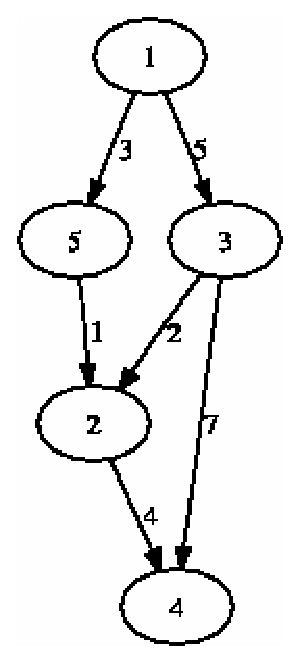
\epsfig{file=graph.eps, scale=0.7}} 
  \caption{A simple weighted directed graph.}
  \label{fig:graph.eps}
\end{figure}


In order to compute the distances from a given node to all other nodes we first have to decide how
to represent a weighted directed graph.  In our implementation of Dijkstra's algorithm we will
assume that the set of nodes $V$ is given as a set of consecutive natural numbers of the form
\\[0.2cm]
\hspace*{1.3cm}
$V = \{ 1, 2, \cdots, n-1, n \}$.
\\[0.2cm]
Therefore, there is no need to store the set $V$.  All we have to store is the number of nodes $n$.
The set of edges $E$ and the function \texttt{length} will be stored using (a variant of) an
\href{http://en.wikipedia.org/wiki/Adjacency_list}{\emph{adjacency list representation}}.
To this end, we define a binary relation \texttt{edges} so that for every node $x \in V$ the
expression \texttt{edges[$x$]} is a set of the form
\\[0.2cm]
\hspace*{1.3cm}
$\texttt{edges[}x\mathtt{]} = \{ \pair(y_1,w_1), \cdots \pair(y_n,w_n) \}$, 
\\[0.2cm]
so that there is an edge form $x$ to $y_i$ for all $i=1,\cdots,n$ and, furthermore, the length of
this edge is $w_i$, i.e.~we have 
\\[0.2cm]
\hspace*{1.3cm}
$\mathtt{length}(\pair(x,y_i)) = w_i$ \quad for all $i=1,\cdots,n$.
\\[0.2cm]
Stated differently, if $x$ and $y$ are nodes in $V$ such that $\pair(x,y)$ is an edge in $E$ of length
$w$, then we have
\\[0.2cm]
\hspace*{1.3cm}
$\pair(y,w) \in \mathtt{edges[}x\mathtt{]}$.
\\[0.2cm]
For example, the relation \texttt{edges} for the graph shown in Figure \ref{fig:graph.eps} can be
defined in \textsc{SetlX} as follows:
\\[0.2cm]
\hspace*{1.3cm}
\texttt{edges := \{ [1, \{[5,3]], [3,5]\}], [5, \{[2,1]\}], \\
\hspace*{3.25cm} 
[3, \{[2,2], [4,7]\}], [2, \{[4,4]\}], [4, \{\}] \};}


\begin{figure}[!ht]
\centering
\begin{Verbatim}[ frame         = lines, 
                  framesep      = 0.3cm, 
                  firstnumber   = 1,
                  labelposition = bottomline,
                  numbers       = left,
                  numbersep     = -0.2cm,
                  xleftmargin   = 0.8cm,
                  xrightmargin  = 0.8cm,
                ]
    class graph(numberNodes, edges) {
        mNumberNodes := numberNodes;
        mEdges       := edges;
    
      static {
        shortestPath := procedure(source) {
            oo   := mathConst("Infinity");
            dist := { [ x, oo ]: x in [1 .. mNumberNodes] };
            dist[source] := 0;
            fringe  := { [0, source] };
            visited := {};
            while (fringe != {}) {
                [d, u] := first(fringe);
                fringe -= { [d, u] };
                for ([v,l] in mEdges[u] | !(v in visited)) {
                    if (d + l < dist[v]) {
                        dvOld := dist[v];
                        dvNew := d + l;
                        dist[v] := dvNew;
                        fringe -= { [dvOld, v] };
                    }
                    fringe += { [dist[v], v] };
                }
                visited += { u };
            }
            return dist;
        };
      }
    }
\end{Verbatim}
\vspace*{-0.3cm}
\caption{A class to represent graphs with an implementation of Dijkstra's algorithm.}
\label{fig:dijkstra.stlx}
\end{figure}

\vspace*{0.3cm}

\noindent
Now we are ready to present Dijkstra's algorithm in \textsc{SetlX}.
Figure \ref{fig:dijkstra.stlx} on page \pageref{fig:dijkstra.stlx} shows the implementation of the
class \texttt{graph} that is used to represent a weighted directed graph.  We discuss the
implementation line by line.
\begin{enumerate}
\item Line 1 starts to define the class \texttt{graph} and the constructor for
      this class.  In \textsc{SetlX}, every class has exactly one constructor and the definition of
      the class and the constructor are the same.  

      In this case, the constructor takes two arguments.  
      \begin{enumerate}
      \item The first argument \texttt{numberNodes}
            specifies the number of nodes.  Implicitly, this argument also specifies the set of nodes
            of the graph since we have agreed that the set of nodes $V$ has the form
            \\[0.2cm]
            \hspace*{1.3cm}
            $V = \{1,2,\cdots, n-1, n\}$.
            \\[0.2cm]
            Therefore, since \texttt{numberNodes} is the number of nodes, we must have 
            $n = \mathtt{numberNodes}$.
      \item The second argument \texttt{edges} specifies both the set of edges and the function
            \texttt{length}  in the way discussed above.
      \end{enumerate}
\item Line 2 and 3 define and assign the member variables \texttt{mNumberNodes} and \texttt{mEdges}.
      Every object $o$ of class \texttt{graph} will therefore have the two attributes
      \texttt{mNumberNodes} and \texttt{mEdges}.  For a given object $o$, these attributes can be
      accessed as $o\mathtt{.mNumberNodes}$ and $o\mathtt{.mEdges}$ respectively.  
      These variables store the number of nodes and the edges in the way discussed previously.
\item Line 5 declares the beginning of a static block which ends in line 28.  
      In this case, the static block contains only the definition of the variable \texttt{shortestPath}.
      Of course, if $o$ is an object of class
      \texttt{graph} then $o\mathtt{.shortestPath}$ will access the function stored in the
      static variable \texttt{shortestPath}.  We defer the discussion of the implementation of this
      function.
\end{enumerate}
At this point, it should be noted that the function \texttt{shortestPath} accesses the variables
\texttt{mNumberNodes} and \texttt{mEdges} 
and these variables are \underline{not} static.  The reason the function \texttt{shortestPath} is
defined \texttt{static} is the fact that the implementation of this function is always the same, no
matter what the graph is.  Therefore, 
there is no need to store this implementation on a per object basis.  Hence, it is sufficient to provide this
function as a static variable of the class \texttt{graph}.  Of course, calling this function as
\\[0.2cm]
\hspace*{1.3cm}
$\texttt{graph.shortestPath}(s)$
\\[0.2cm]
wouldn't make any sense as then the variables \texttt{mNumberNodes} and \texttt{mEdges} would both
be undefined.  In order to call this function, we need to have an object $g$ of class \texttt{graph}.
Then it will make sense to write
\\[0.2cm]
\hspace*{1.3cm}
$g\mathtt{.shortestPath}(s)$
\\[0.2cm]
as in this case the function \texttt{shortestPath} has access to the member variables
\texttt{mNumberNodes} and \texttt{mEdges} that are stored in the object $g$.

Let us now briefly explain the implementation of the function \texttt{shortestPath}.  This function
gets a single node \texttt{source} as its argument and it will compute the distance of all other
nodes from the node \texttt{source}.  This distance will be represented as a binary relation that is stored
in the variable \texttt{dist}.  The elements of this binary relation will be pairs of the form
\\[0.2cm]
\hspace*{1.3cm}
$[x, d]$
\\[0.2cm]
where $x$ is a node and $d$ is the distance of this node.
When given the graph $g$ depicted in Figure \ref{fig:dijkstra.stlx}, the
expression 
\\[0.2cm]
\hspace*{1.3cm}
$g\mathtt{.shortestPath(1)}$
\\[0.2cm]
will yield the result
\\[0.2cm]
\hspace*{1.3cm}
\texttt{\{[1, 0], [2, 4], [3, 5], [5, 3], [4, 8]\}}.
\\[0.2cm]
This elements of this binary relation are to be interpreted as follows:  
\begin{enumerate}
\item The distance of the node $1$ from the node $1$ is obviously $0$.
\item The distance of the node $2$ from the node $1$ is $4$.  
      The path $[1,5,2]$ exhibits this length.
\item $\vdots$
\item The distance of the node $4$ from the node $1$ is $8$.
      The path $[1,5,2,4]$ is the shortest path connecting the node $1$ with the node $4$
      and has length $8$.
\end{enumerate}
The relation \texttt{dist}, which is computed and returned by the function \texttt{shortestPath}, is
initialized in line 8 to assign the distance $\infty$ for every node $x$ of the graph.  This distance
can be seen as an upper estimate of the minimum length of a path connecting the \texttt{source} to
the node $x$.  Since we do not yet know whether the node $x$ is reachable from the node
\texttt{source} at all, we initialize the distance to $\infty$.
Initially, the only node that is definitely reachable from the node \texttt{source} is the node
\texttt{source} itself.  Therefore, \texttt{dist[source]} is set to $0$ in line 9.

The algorithm to compute all distances maintains two data structures.
\begin{enumerate}
\item \texttt{fringe} is the set of those nodes $x$ that have already been encountered when traversing
      the graph, but which have not been fully explored in the sense that there are nodes $y$ such
      that there is an edge $\pair(x,y)$ and the node $y$ has not been visited.
      
      However, instead of just storing these nodes, for every node $y$ the set \texttt{fringe} stores a pair
      of the form 
      \\[0.2cm]
      \hspace*{1.3cm}
      $[w, y]$,
      \\[0.2cm]
      where $w$ is the best estimate of the distance of the node $y$ from the node \texttt{source}.
      Initially, we have only visited the node \texttt{source} and its distance from \texttt{source}
      is obviously $0$.  Therefore, \texttt{fringe} is initialized as
      \\[0.2cm]
      \hspace*{1.3cm}
      \texttt{\{ [0, source] \}}
      \\[0.2cm]
      in line 13.  Since a node $u$ with distance $d$ is stored as the pair $[d, u]$, the set
      \texttt{fringe} can be used as a priority queue.  The reason is that in \textsc{SetlX} every
      set is stored as an ordered binary tree.  Therefore, the elements of a set are ordered and it
      is easy to pick the smallest element of a set using the function \texttt{first}.  
      Since, furthermore, lists (and pairs in
      particular) are ordered lexicographically, the first element in the set \texttt{fringe} is 
      the pair $[d, u]$ with the smallest value of $d$, i.e.~the node $u$ in the set \texttt{fringe}
      that is closest to the \texttt{source}.
\item \texttt{visited} is the set of nodes that habe been \emph{visited} in the following sense:
      A node $x$ is said to have been \emph{visited} if all of the neighbours of $x$, i.e.~all nodes
      $y$ such that there is an edge $\pair(x,y)$ have been inspected and have been assigned a 
      distance.  It may be the case that the distance assigned to $y$ will improve later,
      but once a node $x$ is added to the set \texttt{visited}, the distance of $x$ from
      \texttt{source} is known.  Initially, the set \texttt{visited} is empty.
\end{enumerate}
The workhorse of the function \texttt{shortestPath} is the \texttt{while}-loop in line 12.  As long
as there are nodes $u$ in the \texttt{fringe} we try to improve the estimate $\mathtt{dist}[v]$ for
all nodes $v$ such that there is an edge $\pair(u,v)$ from $u$ to $v$.  The idea is that if 
\\[0.2cm]
\hspace*{1.3cm}
$\mathtt{dist}[u] + l < \mathtt{dist}[v]$, \quad where $l$ is the length of the edge $\pair(u,v)$
\\[0.2cm]
then we can improve our estimate of $\texttt{dist}[v]$ by assigning
\\[0.2cm]
\hspace*{1.3cm}
\texttt{dist[v] := dist[u] + l;}
\\[0.2cm]
After updating the distance of node $v$, we have to add this node to the \texttt{fringe} so that we
can in turn deal with those nodes that are reachable from node $v$.  The thing that makes Dijkstra's
algorithm fast is the fact that once a node is visited we know that its distance can not be improved
in the future.  A proof of this fact can be found in a 
\href{http://www-m3.ma.tum.de/foswiki/pub/MN0506/WebHome/dijkstra.pdf}{paper} of Dijkstra \cite{dijkstra:59}.
\vspace*{0.3cm}

\noindent
\textbf{Remark}:  At this point you might feel a little bit disappointed because the previous example
has not made much use of the object-oriented features of \textsc{SetlX}.  However, that is exactly
the point of this example: Of course we could have implemented graph nodes as object of some class
and do the same for edges.  However, the resulting program would then suffer from code bloat.  We do
not think that object-oriented programming should be used for the sake of object-oriented
programming but rather see it as a convenient method to encapsulate data, nothing more.  In
particular, an object-oriented program is not, in general, better than a program that does not use
object-oriented features.  We therefore advocate to use classes when this is either necessary or 
convenient but not for the sake of object-oriented programming.

\section{Representing Complex Numbers as Objects}
Our next example deals with 
\href{http://en.wikipedia.org/wiki/Complex_number}{\emph{complex numbers}}.  
Remember that complex numbers have the form
\\[0.2cm]
\hspace*{1.3cm}
$z = x + y \cdot i$, \quad where $x,y \in \mathbb{R}$ and $i \cdot i = -1$.
\\[0.2cm]
Assume that we have to perform a number of intricate calculations using complex numbers.  One way
we could do this is by representing a complex number $x + y \cdot i$ as a pair $[x,y]$.  Then we
would have to implement functions to add, subtract, multiply,  and divide complex numbers.  For
example, methods to add and multiply two complex numbers would have the following form: 

\begin{figure}[!ht]
\centering
\begin{Verbatim}[ frame         = lines, 
                  framesep      = 0.3cm, 
                  firstnumber   = 1,
                  labelposition = bottomline,
                  numbers       = left,
                  numbersep     = -0.2cm,
                  xleftmargin   = 0.8cm,
                  xrightmargin  = 0.8cm,
                ]
    addComplex := procedure(z1, z2) {
        [x1, y1] := z1;
        [x2, y2] := z2;
        return [x1 + x2, y1 + y2];	
    }; 
    multiplyComplex := procedure(z1, z2) {
        [x1, y1] := z1;
        [x2, y2] := z2;
        return [x1*x2 - y1*y2, x1*y2 + x2*y1];	
    }; 
\end{Verbatim}
\vspace*{-0.3cm}
\caption{Representing complex numbers as pairs.}
\label{fig:add-complex.stlx}
\end{figure}


\begin{figure}[!ht]
\centering
\begin{Verbatim}[ frame         = lines, 
                  framesep      = 0.3cm, 
                  labelposition = bottomline,
                  numbers       = left,
                  numbersep     = -0.2cm,
                  xleftmargin   = 0.0cm,
                  xrightmargin  = 0.0cm,
                ]
    class complex(real, imag) {
        mReal := real;
        mImag := imag;
      static {    
        sum := 
            that |-> complex(mReal + that.mReal, mImag + that.mImag);
        difference := 
            that |-> complex(mReal - that.mReal, mImag - that.mImag);
        product := procedure(that) {
            return complex(mReal * that.mReal - mImag * that.mImag,
                           mReal * that.mImag + mImag * that.mReal);
        };
        quotient := procedure(that) {
            denom := that.mReal * that.mReal + mImag * mImag;
            real  := (mReal * that.mReal + mImag * that.mImag) / denom;
            imag  := (mImag * that.mReal - mReal * that.mImag) / denom;
            return complex(real, imag);
        };
        power := procedure(that) {
            return exp(that * log(this));
        };
        f_exp := procedure() {
            r := exp(mReal);
            return complex(r * cos(mImag), r * sin(mImag));
        };
        f_log := procedure() {
            r := log(mReal * mReal + mImag * mImag) / 2; 
            return complex(r, atan2(mImag, mReal));
        };
        f_str := [] |-> mReal + " + " + mImag + " * i";
        equals := procedure(that) {
            return mReal == that.mReal && mImag == that.mImag;
        };
      }
    }
\end{Verbatim}
\vspace*{-0.3cm}
\caption{The class \texttt{complex} implementing complex numbers.}
\label{fig:complex.stlx}
\end{figure}

While it is certainly possible to represent complex numbers in this way, this method is not very convenient.
One reason is that a even a moderately sized formula involving complex numbers would be more or less unreadable 
when implemented using functions like \texttt{addComplex} and \texttt{multiplyComplex}.  Fortunately, there is 
a better way to represent complex numbers in \textsc{SetlX}.  Figure \ref{fig:complex.stlx} shows how we can define
the class \texttt{complex} that represents complex numbers.  In fact, \texttt{complex} is both a class and a 
\emph{constructor} for this class.  This constructor takes two arguments:
\begin{enumerate}
\item \texttt{real} is the real part of the complex number that is represented, while
\item \texttt{imag} is the imaginary part.
\end{enumerate}
The class complex has two \emph{member variables}.  These member variables are called \texttt{mReal} and \texttt{mImag}.
These member variables are defined and initialized in lines 2 and 3.  Therefore every object $o$ of class complex stores two 
numbers that can be accessed as
\\[0.2cm]
\hspace*{1.3cm}
\texttt{o.mReal} \quad and \quad \texttt{o.mImag}.
\\[0.2cm]
In order to work with complex numbers we need methods to perform the basic arithmetic operations.
The class \texttt{complex} in Figure \ref{fig:complex.stlx} provides the implementation of functions
to add, subtract, multiply, and divide complex numbers.  As these functions are not properies of a
specific complex number but rather apply to all complex numbers, these functions are defined as
\emph{static members} of the class \texttt{complex}.  We refer to these functions as methods and discuss 
them next.
\begin{enumerate}
\item First, line 5 defines a method called \texttt{sum}.  Despite the looks of it, this
      method takes two arguments.  The first argument is implicit and it is called
      \texttt{this}.  This argument is a reference to an object of class \texttt{complex}.
      The second argument, which we have called \texttt{that}, also references an object
      of class \texttt{complex}.  Now in order to add the complex numbers \texttt{this}
      and \texttt{that} we could just return a new complex number as follows:
      \\[0.2cm]
      \hspace*{1.3cm}
      \texttt{complex(this.mReal + that.mReal, this.mImag + that.mImag);}
      \\[0.2cm]
      However, as \texttt{this} is always implicit, the actual implementation of the
      method \texttt{sum} is even simpler and we can instead write
      \\[0.2cm]
      \hspace*{1.3cm}
      \texttt{complex(mReal + that.mReal, mImag + that.mImag);}
      \\[0.2cm]
      to create a complex number that is the sum of the complex number \texttt{this} and
      \texttt{that}.

      In order to invoke the method \texttt{sum}, let us first create two complex numbers
      \texttt{z1} and \texttt{z2} as follows:      
      \\[0.2cm]
      \hspace*{1.3cm}
      \texttt{z1 := complex(1,2);}
      \\
      \hspace*{1.3cm}
      \texttt{z2 := complex(3,1);}
      \\[0.2cm]
      Now we have $\mathtt{z1} = 1 + 2 \cdot i$ and $\mathtt{z2} = 3 + 1 \cdot i$.  In
      order to add these numbers, we can execute the assignment
      \\[0.2cm]
      \hspace*{1.3cm}
      \texttt{z3 := z1.sum(z2);}
      \\[0.2cm]
      This will set \texttt{z3} to the complex number $4 + 3 \cdot i$.  Fortunately, as
      \textsc{SetlX} supports operator overloading, we can write
      \\[0.2cm]
      \hspace*{1.3cm}
      \texttt{z3 := z1 + z2;}
      \\[0.2cm]
      in order to compute the sum of \texttt{z1} and \texttt{z2}.  

      \textbf{Note}:  For operator overloading to work out we have to use the same method
      name that is used when \textsc{SetlX} evaluates the corresponding operator.  
      For the operator ``\texttt{+}'' performing addition, the corresponding name
      is \texttt{sum}.  Table \ref{tab:operator-names} lists the names corresponding to the operators
      provided by \textsc{SetlX}.  Note that certain operators cannot be overloaded because they are
      implicitly reduced to other operators.  In particular
      \begin{enumerate}
      \item \texttt{a <==> b} \quad is reduced to \quad \texttt{a == b},
      \item \texttt{a <!=> b} \quad is reduced to \quad \texttt{!(a == b)},
      \item \texttt{a != b} \quad is reduced to \quad \texttt{!(a == b)},
      \item \texttt{a <= b} \quad is reduced to \quad \texttt{a == b || a < b},
      \item \texttt{a >= b} \quad is reduced to \quad \texttt{a == b || b < a}, \quad and
      \item \texttt{a > \ b} \quad is reduced to \quad \texttt{b < a}.
      \end{enumerate}
      Furthermore, the operators ``\texttt{+/}'' and ``\texttt{*/}'' are reduced to applications of
      the operators ``\texttt{+}'' and ``\texttt{*}''.  Therefore, it does not make sense to
      overload these operators on their own.  They are implictitly overloaded when the operators 
      ``\texttt{+}'' and ``\texttt{*}'' are overloaded.
      \begin{table}[!hbt]
        \centering
        \begin{tabular}[t]{|l|l||l|l|}
          \hline
          Operator    & Name  & Operator & Name \\
          \hline
          \hline
          \texttt{+}  & \texttt{sum}         & \texttt{\symbol{38}\symbol{38}}  & \texttt{conjunction} \\
          \hline
          \texttt{-}  & \texttt{difference}  & \texttt{\symbol{124}\symbol{124}}  & \texttt{disjunction} \\
          \hline
          \texttt{*}  & \texttt{product}  & \texttt{=>}  & \texttt{implication} \\
          \hline
          \texttt{/}  & \texttt{quotient}    & \texttt{==}  & \texttt{equals} \\
          \hline
          \texttt{\%}  & \texttt{modulo}     & \texttt{**}  & \texttt{power}  \\
          \hline
          \texttt{\symbol{92}}  & \texttt{integerDivision}    & \texttt{<}  & \texttt{lessThan}   \\
          \hline
          \texttt{><}  & \texttt{cartesianProduct}    &   &    \\
          \hline
        \end{tabular}

        \caption{Operator names.}
        \label{tab:operator-names}
      \end{table}
      
      In case you want to find the names of these operators by yourself and do not have access to
      this manual, then there is a neat trick to figure out these names.  Define the class
      \texttt{empty} as
      \\[0.2cm]
      \hspace*{1.3cm}
      \texttt{class empty() \{\}}
      \\[0.2cm]
      Then, evaluating the expression
      \\[0.2cm]
      \hspace*{1.3cm}
      \texttt{a == a}
      \\[0.2cm]
      will result in the error message
      \\[0.2cm]
      \hspace*{1.3cm}
      \texttt{Error in "a == a":}       \\
      \hspace*{1.3cm}
      \texttt{Member 'equals' is undefined in 'object<\{ class () \{\} \}>'.}
      \\[0.2cm]
      This message shows that the operator \texttt{==} has the name ``\texttt{equals}''.  Evaluating
      the expression
      \\[0.2cm]
      \hspace*{1.3cm}
      \texttt{a <= a;}
      \\[0.2cm]
      yields the error message
      \\[0.2cm]
      \hspace*{1.3cm}
      \texttt{Error in "a <= a":} \\
      \hspace*{1.3cm}
      \texttt{Error in substitute comparison "(a == a) || (a < a)":} \\
      \hspace*{1.3cm}
      \texttt{Member 'equals' is undefined in 'object<{ class () {  } }>'.}
      \\[0.2cm]
      This error message shows that the expression ``\texttt{a <= b}'' is reduced to the expression \\
      ``\texttt{(a == b) || (a < b)}''.

      Finally, note that Table \ref{tab:operator-names} only lists the binary operators.  
      There are three unary operators that can be overloaded, too.
      \begin{enumerate}
      \item The operator ``\texttt{-}'' has the name ``\texttt{minus}'' when used as a unary prefix
            operator. 
      \item The operator ``\texttt{!}'' has the name ``\texttt{not}'' when used as a unary prefix
            operator.  This same operator has the name ``\texttt{factorial}'' when used as a unary
            postfix operator.
      \end{enumerate}
\item The implementation of the method \texttt{difference} in line 7 and 8 is similar to
      the implementation of \texttt{sum}.
\item The method \texttt{product} in line 9 takes two objects of class \texttt{complex}
      and computes their product according to the formula
      \\[0.2cm]
      \hspace*{1.3cm}
      $(x_1 + y_1 \cdot i) \cdot (x_2 + y_2 \cdot i) = 
       x_1 \cdot x_2 - y_1 \cdot y_2 + (x_1 \cdot y_2 + x_2 \cdot y_1) \cdot i
      $.
      \\[0.2cm]
      Instead of the ``\texttt{|->}''-notation used to define the methods \texttt{sum} and
      \texttt{difference} we have defined these methods via the keyword
      ``\texttt{procedure}''.  Defining this method via ``\texttt{procedure}'' is more
      convenient as the implementation of the method requires more than one line.
      As a rule of thumb, we recommend using the ``\texttt{|->}''-notation only in cases
      where the body of a function fits into a single line.
\item The method \texttt{quotient} in line 13 implements the division of complex numbers
      according to the formula
      \\[0.2cm]
      \hspace*{1.3cm}
      ${\displaystyle\; x_1 + y_1 \cdot i \;\over \displaystyle x_2 + y_2 \cdot i} = 
       {\displaystyle\; x_1 \cdot x_2 + y_1 \cdot y_2 \;\over \displaystyle x_2 \cdot x_2 + y_2 \cdot y_1} +
       {\displaystyle\; y_1 \cdot x_2 - x_1 \cdot y_2 \;\over \displaystyle x_2 \cdot x_2 + y_2 \cdot y_1} \cdot i
      $.
\item The method \texttt{power} raises the complex number \texttt{this} to the power of
      the argument \texttt{that}.  This is done with the help of the function
      \texttt{exp} and \texttt{log} via the equation
      \\[0.2cm]
      \hspace*{1.3cm}
      $z_1^{z_2} = \mathtt{exp}(z_2 \cdot \mathtt{log}(z_1))$.
      \\[0.2cm]
      Of course, for this to work we need to implement the functions \texttt{exp} and
      \texttt{log} for complex numbers.
\item Line 22 defines the function ``\texttt{f\_exp}''.  Note that this function is not
      called ``\texttt{exp}'' but is rather called ``\texttt{f\_exp}''.  In
      \textsc{SetlX}, if we want to redefine a predefined function like the function
      ``\texttt{exp}'' we have to put the string ``\texttt{f\_}'' in front of the function
      name.  Later, when we invoke the function, the prefix ``\texttt{f\_}'' is dropped.
      For example, if we want to compute the exponential of the imaginary unit $i$ we can
      define
      \\[0.2cm]
      \hspace*{1.3cm}
      \texttt{i := complex(0,1);}
      \\[0.2cm]
      and can then invoke the exponential function as
      \\[0.2cm]
      \hspace*{1.3cm}
      \texttt{exp(i);}
      \\[0.2cm]
      The exponential of a complex number $z = x + y \cdot i$ is computed according to
      \href{http://en.wikipedia.org/wiki/Euler%27s_formula}{Euler's formula} as
      \\[0.2cm]
      \hspace*{1.3cm}
      $\exp(x + y \cdot i) = exp(x) \cdot \bigl(\cos(y) + \sin(y) \cdot i\bigr)$.
\item Line 22 defines a function to compute the natural logarithm of a complex number $z$.
      In order to compute the natural logarithm of the complex number $z = x + y \cdot i$ we rewrite $z$
      in polar coordinates so that $z = r \cdot e^{\varphi \cdot i}$.   Here, $r$ and
      $\varphi$ are given as
      \\[0.2cm]
      \hspace*{1.3cm}
      $r = \sqrt{x^2 + y^2}$ \quad and \quad $\varphi = \mathtt{atan2}(y, x)$.
      \\[0.2cm]
      Then we have
      \\[0.2cm]
      \hspace*{1.3cm}
      $\log(z) = \log\bigl(r \cdot e^{\varphi \cdot i}\bigr) = \log r + \varphi \cdot i$.
\item Line 30 defines a function that converts a complex number into a string.  If a class
      $C$ provides a method with the name ``\texttt{f\_str}'', then everytime that an object
      of class $C$ needs to be converted into a string this function is called implicitly.

\item Finally, we define the method \texttt{equals} in line 31.  This method is automatically
      invoked when two objects of class \texttt{complex} are compared using either the
      operator ``\texttt{==}'' or the operator ``\texttt{!=}''.
\item Unfortunately, it does not make sense to define the operator ``\texttt{<}'' for complex
      numbers.  Therefore, this operator has not been overloaded.
\end{enumerate}


                
 
%%% Local Variables: 
%%% mode: latex
%%% TeX-master: "tutorial"
%%% End: 
